\documentclass[a4paper]{book}
\usepackage{a4wide}
\usepackage{makeidx}
\usepackage{fancyhdr}
\usepackage{graphicx}
\usepackage{multicol}
\usepackage{float}
\usepackage{textcomp}
\usepackage{alltt}
\usepackage{times}
\usepackage{ifpdf}
\ifpdf
\usepackage[pdftex,
            pagebackref=true,
            colorlinks=true,
            linkcolor=blue,
            unicode
           ]{hyperref}
\else
\usepackage[ps2pdf,
            pagebackref=true,
            colorlinks=true,
            linkcolor=blue,
            unicode
           ]{hyperref}
\usepackage{pspicture}
\fi
\usepackage[utf8]{inputenc}
\usepackage{doxygen}
\makeindex
\setcounter{tocdepth}{1}
\renewcommand{\footrulewidth}{0.4pt}
\begin{document}
\begin{titlepage}
\vspace*{7cm}
\begin{center}
{\Large UPC Lookup Reference Manual}\\
\vspace*{1cm}
{\large Generated by Doxygen 1.5.3}\\
\vspace*{0.5cm}
{\small Sun Apr 20 19:57:15 2008}\\
\end{center}
\end{titlepage}
\clearemptydoublepage
\pagenumbering{roman}
\tableofcontents
\clearemptydoublepage
\pagenumbering{arabic}
\chapter{UPC Lookup Main Page}
\label{index}\hypertarget{index}{}\begin{Desc}
\item[\hyperlink{todo__todo000001}{Todo}]Make this support everyhting Image\_\-Barcode supports:\begin{itemize}
\item Code 39\item Code 128\item EAN 13\item INT 25\item PostNet\item UPCA \end{itemize}


Fix errors 

Add possible product images 

Move Info output to seperate function\end{Desc}
\begin{Desc}
\item[Version:]0.1 \end{Desc}
\begin{Desc}
\item[Author:]Dan Keenan - \href{http://dankeenan.org}{\tt http://dankeenan.org} \end{Desc}
\hypertarget{index_license}{}\section{License}\label{index_license}
Copyright (C) 2008 Dan Keenan

This program is free software: you can redistribute it and/or modify it under the terms of the GNU General Public License as published by the Free Software Foundation, either version 3 of the License, or (at your option) any later version.

This program is distributed in the hope that it will be useful, but WITHOUT ANY WARRANTY; without even the implied warranty of MERCHANTABILITY or FITNESS FOR A PARTICULAR PURPOSE. See the GNU General Public License for more details.

You should have received a copy of the GNU General Public License along with this program. If not, see $<$\href{http://www.gnu.org/licenses/}{\tt http://www.gnu.org/licenses/}$>$.



A \hyperlink{license}{full text } of this license is available 
\chapter{UPC Lookup Class Index}
\section{UPC Lookup Class List}
Here are the classes, structs, unions and interfaces with brief descriptions:\begin{CompactList}
\item\contentsline{section}{\hyperlink{classXML}{XML} }{\pageref{classXML}}{}
\end{CompactList}

\chapter{UPC Lookup File Index}
\section{UPC Lookup File List}
Here is a list of all files with brief descriptions:\begin{CompactList}
\item\contentsline{section}{\hyperlink{index_8php}{index.php} (Main handler file, contains all HTML code )}{\pageref{index_8php}}{}
\item\contentsline{section}{\hyperlink{upcimg_8php}{upcimg.php} (Creates an image of the barcode using Image\_\-Barcode )}{\pageref{upcimg_8php}}{}
\item\contentsline{section}{include/\hyperlink{barcode_8inc}{barcode.inc} (Functions for the handling of different barcodes )}{\pageref{barcode_8inc}}{}
\item\contentsline{section}{include/\hyperlink{form_8inc}{form.inc} (Functions for outputting the Barcode entry form )}{\pageref{form_8inc}}{}
\item\contentsline{section}{include/\hyperlink{pear_8inc}{pear.inc} (Makes PEAR work with extentions installed in the home directory )}{\pageref{pear_8inc}}{}
\item\contentsline{section}{include/\hyperlink{product_8inc}{product.inc} (Functions to output Product Info )}{\pageref{product_8inc}}{}
\item\contentsline{section}{include/\hyperlink{utils_8inc}{utils.inc} (Helpful Utilities )}{\pageref{utils_8inc}}{}
\item\contentsline{section}{include/\hyperlink{xmlrpc_8inc}{xmlrpc.inc} (XML-RPC Library )}{\pageref{xmlrpc_8inc}}{}
\end{CompactList}

\chapter{UPC Lookup Page Index}
\section{UPC Lookup Related Pages}
Here is a list of all related documentation pages:\begin{CompactList}
\item \contentsline{section}{Todo List}{\pageref{todo}}{}

\item \contentsline{section}{License}{\pageref{license}}{}

\item \contentsline{section}{Google AJAX Search API}{\pageref{searchapi}}{}

\end{CompactList}

\chapter{UPC Lookup Class Documentation}
\hypertarget{classXML}{
\section{XML Class Reference}
\label{classXML}\index{XML@{XML}}
}
\subsection*{Public Member Functions}
\begin{CompactItemize}
\item 
\hyperlink{classXML_1475a1374023931e2227277f4047c9aa}{XML} (\$data=null)
\item 
\hyperlink{classXML_d1524d80c783b2cd22966462411b9b7d}{destruct} ()
\item 
\hyperlink{classXML_61e6258dc3d5750100e1f0dd08d6334a}{parse} (\$data)
\item 
\hyperlink{classXML_eac7eae74d866d4f5a0cdb9be27ff279}{open} (\$parser, \$tag, \$attributes)
\item 
\hyperlink{classXML_ca70dfbd3e8ce956075181701b09b033}{data} (\$parser, \$data)
\item 
\hyperlink{classXML_60144a2134fc1b7f5b4b1b6a7c56bf04}{close} (\$parser, \$tag)
\end{CompactItemize}
\subsection*{Public Attributes}
\begin{CompactItemize}
\item 
\hyperlink{classXML_fa14fbca44236b30ab5f3dcfc4b02890}{\$parser}
\item 
\hyperlink{classXML_01d565098eeda8bf09e4242a2748d570}{\$document}
\item 
\hyperlink{classXML_7c20d75c1719294f3320a537a32753ca}{\$current}
\item 
\hyperlink{classXML_fa51193c2f0b317f817fa3efa8722227}{\$parent}
\item 
\hyperlink{classXML_c10be009a77c59e80ce5562d4dd35532}{\$parents}
\item 
\hyperlink{classXML_60e7e74df6643f50e0c6ea8252554b3d}{\$last\_\-opened\_\-tag}
\end{CompactItemize}


\subsection{Detailed Description}


Definition at line 72 of file xmlrpc.inc.

\subsection{Member Function Documentation}
\hypertarget{classXML_1475a1374023931e2227277f4047c9aa}{
\index{XML@{XML}!XML@{XML}}
\index{XML@{XML}!XML@{XML}}
\subsubsection{\setlength{\rightskip}{0pt plus 5cm}XML::XML (\$ {\em data} = {\tt null})}}
\label{classXML_1475a1374023931e2227277f4047c9aa}




Definition at line 81 of file xmlrpc.inc.

\begin{Code}\begin{verbatim}81                           {
82     $this->parser = xml_parser_create();
83 
84     xml_parser_set_option ($this->parser, XML_OPTION_CASE_FOLDING, 0);
85     xml_set_object($this->parser, &$this);
86     xml_set_element_handler($this->parser, "open", "close");
87     xml_set_character_data_handler($this->parser, "data");
88 #   register_shutdown_function(array(&$this, 'destruct'));
89   }
\end{verbatim}
\end{Code}


\hypertarget{classXML_d1524d80c783b2cd22966462411b9b7d}{
\index{XML@{XML}!destruct@{destruct}}
\index{destruct@{destruct}!XML@{XML}}
\subsubsection{\setlength{\rightskip}{0pt plus 5cm}XML::destruct ()}}
\label{classXML_d1524d80c783b2cd22966462411b9b7d}




Definition at line 91 of file xmlrpc.inc.

\begin{Code}\begin{verbatim}91                      {
92     xml_parser_free($this->parser);
93   }
\end{verbatim}
\end{Code}


\hypertarget{classXML_61e6258dc3d5750100e1f0dd08d6334a}{
\index{XML@{XML}!parse@{parse}}
\index{parse@{parse}!XML@{XML}}
\subsubsection{\setlength{\rightskip}{0pt plus 5cm}XML::parse (\$ {\em data})}}
\label{classXML_61e6258dc3d5750100e1f0dd08d6334a}




Definition at line 95 of file xmlrpc.inc.

\begin{Code}\begin{verbatim}95                        {
96     $this->document = array();
97     $this->parent = &$this->document;
98     $this->parents = array();
99     $this->last_opened_tag = NULL;
100     xml_parse($this->parser, $data);
101     return $this->document;
102   }
\end{verbatim}
\end{Code}


\hypertarget{classXML_eac7eae74d866d4f5a0cdb9be27ff279}{
\index{XML@{XML}!open@{open}}
\index{open@{open}!XML@{XML}}
\subsubsection{\setlength{\rightskip}{0pt plus 5cm}XML::open (\$ {\em parser}, \$ {\em tag}, \$ {\em attributes})}}
\label{classXML_eac7eae74d866d4f5a0cdb9be27ff279}




Definition at line 104 of file xmlrpc.inc.

References count\_\-numeric\_\-items(), and data().

\begin{Code}\begin{verbatim}104                                            {
105     #echo "Opening tag $tag<br>\n";
106     $this->data = "";
107     $this->last_opened_tag = $tag; #tag is a string
108     if(array_key_exists($tag, $this->parent)){
109       #echo "There's already an instance of '$tag' at the current level ($level)<br>\n";
110       if(is_array($this->parent[$tag]) and array_key_exists(0, $this->parent[$tag])){ #if the keys are numeric
111         #need to make sure they're numeric (account for attributes)
112         $key = count_numeric_items($this->parent[$tag]);
113         #echo "There are $key instances: the keys are numeric.<br>\n";
114       }else{
115         #echo "There is only one instance. Shifting everything around<br>\n";
116         $temp = &$this->parent[$tag];
117         unset($this->parent[$tag]);
118         $this->parent[$tag][0] = &$temp;
119 
120         if(array_key_exists("$tag attr", $this->parent)){
121           #shift the attributes around too if they exist
122           $temp = &$this->parent["$tag attr"];
123           unset($this->parent["$tag attr"]);
124           $this->parent[$tag]["0 attr"] = &$temp;
125         }
126         $key = 1;
127       }
128       $this->parent = &$this->parent[$tag];
129     }else{
130       $key = $tag;
131     }
132     if($attributes){
133       $this->parent["$key attr"] = $attributes;
134     }
135 
136     $this->parent[$key] = array();
137     $this->parent = &$this->parent[$key];
138     array_unshift($this->parents, &$this->parent);
139   }
\end{verbatim}
\end{Code}




Here is the call graph for this function:\nopagebreak
\begin{figure}[H]
\begin{center}
\leavevmode
\includegraphics[width=134pt]{classXML_eac7eae74d866d4f5a0cdb9be27ff279_cgraph}
\end{center}
\end{figure}
\hypertarget{classXML_ca70dfbd3e8ce956075181701b09b033}{
\index{XML@{XML}!data@{data}}
\index{data@{data}!XML@{XML}}
\subsubsection{\setlength{\rightskip}{0pt plus 5cm}XML::data (\$ {\em parser}, \$ {\em data})}}
\label{classXML_ca70dfbd3e8ce956075181701b09b033}




Definition at line 141 of file xmlrpc.inc.

Referenced by close(), and open().

\begin{Code}\begin{verbatim}141                                {
142     #echo "Data is '", htmlspecialchars($data), "'<br>\n";
143     if($this->last_opened_tag != NULL){
144       $this->data .= $data;
145     }
146   }
\end{verbatim}
\end{Code}




Here is the caller graph for this function:\nopagebreak
\begin{figure}[H]
\begin{center}
\leavevmode
\includegraphics[width=107pt]{classXML_ca70dfbd3e8ce956075181701b09b033_icgraph}
\end{center}
\end{figure}
\hypertarget{classXML_60144a2134fc1b7f5b4b1b6a7c56bf04}{
\index{XML@{XML}!close@{close}}
\index{close@{close}!XML@{XML}}
\subsubsection{\setlength{\rightskip}{0pt plus 5cm}XML::close (\$ {\em parser}, \$ {\em tag})}}
\label{classXML_60144a2134fc1b7f5b4b1b6a7c56bf04}




Definition at line 148 of file xmlrpc.inc.

References data().

\begin{Code}\begin{verbatim}148                                {
149     #echo "Close tag $tag<br>\n";
150     if($this->last_opened_tag == $tag){
151       $this->parent = $this->data;
152       $this->last_opened_tag = NULL;
153     }
154     array_shift($this->parents);
155     $this->parent = &$this->parents[0];
156   }
\end{verbatim}
\end{Code}




Here is the call graph for this function:\nopagebreak
\begin{figure}[H]
\begin{center}
\leavevmode
\includegraphics[width=107pt]{classXML_60144a2134fc1b7f5b4b1b6a7c56bf04_cgraph}
\end{center}
\end{figure}


\subsection{Member Data Documentation}
\hypertarget{classXML_fa14fbca44236b30ab5f3dcfc4b02890}{
\index{XML@{XML}!$parser@{\$parser}}
\index{$parser@{\$parser}!XML@{XML}}
\subsubsection{\setlength{\rightskip}{0pt plus 5cm}XML::\$parser}}
\label{classXML_fa14fbca44236b30ab5f3dcfc4b02890}




Definition at line 73 of file xmlrpc.inc.\hypertarget{classXML_01d565098eeda8bf09e4242a2748d570}{
\index{XML@{XML}!$document@{\$document}}
\index{$document@{\$document}!XML@{XML}}
\subsubsection{\setlength{\rightskip}{0pt plus 5cm}XML::\$document}}
\label{classXML_01d565098eeda8bf09e4242a2748d570}




Definition at line 74 of file xmlrpc.inc.\hypertarget{classXML_7c20d75c1719294f3320a537a32753ca}{
\index{XML@{XML}!$current@{\$current}}
\index{$current@{\$current}!XML@{XML}}
\subsubsection{\setlength{\rightskip}{0pt plus 5cm}XML::\$current}}
\label{classXML_7c20d75c1719294f3320a537a32753ca}




Definition at line 75 of file xmlrpc.inc.\hypertarget{classXML_fa51193c2f0b317f817fa3efa8722227}{
\index{XML@{XML}!$parent@{\$parent}}
\index{$parent@{\$parent}!XML@{XML}}
\subsubsection{\setlength{\rightskip}{0pt plus 5cm}XML::\$parent}}
\label{classXML_fa51193c2f0b317f817fa3efa8722227}




Definition at line 76 of file xmlrpc.inc.\hypertarget{classXML_c10be009a77c59e80ce5562d4dd35532}{
\index{XML@{XML}!$parents@{\$parents}}
\index{$parents@{\$parents}!XML@{XML}}
\subsubsection{\setlength{\rightskip}{0pt plus 5cm}XML::\$parents}}
\label{classXML_c10be009a77c59e80ce5562d4dd35532}




Definition at line 77 of file xmlrpc.inc.\hypertarget{classXML_60e7e74df6643f50e0c6ea8252554b3d}{
\index{XML@{XML}!$last_opened_tag@{\$last\_\-opened\_\-tag}}
\index{$last_opened_tag@{\$last\_\-opened\_\-tag}!XML@{XML}}
\subsubsection{\setlength{\rightskip}{0pt plus 5cm}XML::\$last\_\-opened\_\-tag}}
\label{classXML_60e7e74df6643f50e0c6ea8252554b3d}




Definition at line 79 of file xmlrpc.inc.

The documentation for this class was generated from the following file:\begin{CompactItemize}
\item 
include/\hyperlink{xmlrpc_8inc}{xmlrpc.inc}\end{CompactItemize}

\chapter{UPC Lookup File Documentation}
\hypertarget{general_8dox}{
\section{Coding/upc/general.dox File Reference}
\label{general_8dox}\index{Coding/upc/general.dox@{Coding/upc/general.dox}}
}

\hypertarget{index_8php}{
\section{Coding/upc/index.php File Reference}
\label{index_8php}\index{Coding/upc/index.php@{Coding/upc/index.php}}
}
\subsection*{Variables}
\begin{CompactItemize}
\item 
\hyperlink{index_8php_85ae3e64cd40e9564adceb010085e9dd}{\$debug} = TRUE
\end{CompactItemize}


\subsection{Detailed Description}
Returns info on a given UPC Barcode \begin{Desc}
\item[\hyperlink{todo__todo000001}{Todo}]Make this support everyhting Image\_\-Barcode supports:\begin{itemize}
\item Code 39\item Code 128\item EAN 13\item INT 25\item PostNet\item UPCA \end{itemize}


Fix errors \end{Desc}


Definition in file \hyperlink{index_8php-source}{index.php}.

\subsection{Variable Documentation}
\hypertarget{index_8php_85ae3e64cd40e9564adceb010085e9dd}{
\index{index.php@{index.php}!$debug@{\$debug}}
\index{$debug@{\$debug}!index.php@{index.php}}
\subsubsection{\setlength{\rightskip}{0pt plus 5cm}\$debug = TRUE}}
\label{index_8php_85ae3e64cd40e9564adceb010085e9dd}




Definition at line 20 of file index.php.

Referenced by XMLRPC\_\-debug\_\-print().
\hypertarget{pear_8inc}{
\section{include/pear.inc File Reference}
\label{pear_8inc}\index{include/pear.inc@{include/pear.inc}}
}
Makes PEAR work with extentions installed in the home directory. 

\subsection*{Enumerations}
\begin{CompactItemize}
\item 
enum \hyperlink{pear_8inc_d1f917c6039930c80bb1047ae2715e08}{HOME\_\-PEAR\_\-DIR} 
\end{CompactItemize}


\subsection{Detailed Description}
Makes PEAR work with extentions installed in the home directory. 

Most shared hosts do not allow user installation of system-wide PEAR extentions, so this file allows it to work with extentions installed in the user's home directory. To make this work, you need to set the HOME\_\-PEAR\_\-DIR constant to the path where your PEAR extentions are installed. See that documentation for more info. 

Definition in file \hyperlink{pear_8inc-source}{pear.inc}.

\subsection{Enumeration Type Documentation}
\hypertarget{pear_8inc_d1f917c6039930c80bb1047ae2715e08}{
\index{pear.inc@{pear.inc}!HOME_PEAR_DIR@{HOME\_\-PEAR\_\-DIR}}
\index{HOME_PEAR_DIR@{HOME\_\-PEAR\_\-DIR}!pear.inc@{pear.inc}}
\subsubsection{\setlength{\rightskip}{0pt plus 5cm}enum {\bf HOME\_\-PEAR\_\-DIR}}}
\label{pear_8inc_d1f917c6039930c80bb1047ae2715e08}


The location of PEAR extentions in the home directory. This is usually {\bf /home/$<$username$>$/pear/php} 

Definition at line 16 of file pear.inc.
\hypertarget{upcimg_8php}{
\section{upcimg.php File Reference}
\label{upcimg_8php}\index{upcimg.php@{upcimg.php}}
}


\subsection{Detailed Description}
Creates an image of the barcode using Image\_\-Barcode \begin{Desc}
\item[See also:]\href{http://pear.php.net/package/Image_Barcode}{\tt http://pear.php.net/package/Image\_\-Barcode} 

\href{http://pear.php.net/manual/en/package.images.image-barcode.php}{\tt http://pear.php.net/manual/en/package.images.image-barcode.php} \end{Desc}


Definition in file \hyperlink{upcimg_8php-source}{upcimg.php}.
\hypertarget{xmlrpc_8inc}{
\section{Coding/upc/xmlrpc.inc File Reference}
\label{xmlrpc_8inc}\index{Coding/upc/xmlrpc.inc@{Coding/upc/xmlrpc.inc}}
}
\subsection*{Classes}
\begin{CompactItemize}
\item 
class \hyperlink{classXML}{XML}
\end{CompactItemize}
\subsection*{Functions}
\begin{CompactItemize}
\item 
\& \hyperlink{xmlrpc_8inc_a1e9b05a06f28fabb86c10129f5890ef}{XML\_\-serialize} (\&\$data, \$level=0, \$prior\_\-key=NULL)
\item 
\& \hyperlink{xmlrpc_8inc_ef8f3de498a12b230d049cdee6a25145}{XML\_\-unserialize} (\&\$xml)
\item 
\& \hyperlink{xmlrpc_8inc_708b2136ca600664d2207a511b3cf3f8}{XMLRPC\_\-parse} (\&\$request)
\item 
\& \hyperlink{xmlrpc_8inc_c13be54b26e0803d8745e4f019dcfd8a}{XMLRPC\_\-prepare} (\$data, \$type=NULL)
\item 
\& \hyperlink{xmlrpc_8inc_d936fe41ae9c3e0b90bd72ffe82a2969}{XMLRPC\_\-adjustValue} (\&\$current\_\-node)
\item 
\hyperlink{xmlrpc_8inc_ce4ea8e1274ca2ee3f51ec5a724f00f3}{XMLRPC\_\-getParams} (\$request)
\item 
\hyperlink{xmlrpc_8inc_70efa062e92a380196ed8053850c0906}{XMLRPC\_\-getMethodName} (\$methodCall)
\item 
\hyperlink{xmlrpc_8inc_3a98b6984b8ca01752d1aa9a267526a3}{XMLRPC\_\-request} (\$site, \$location, \$methodName, \$params=NULL, \$user\_\-agent=NULL)
\item 
\hyperlink{xmlrpc_8inc_c736d378caaccdd0726ea1080d1f526f}{XMLRPC\_\-response} (\$return\_\-value, \$server=NULL)
\item 
\hyperlink{xmlrpc_8inc_0cdc54b1376ccbbe412175c9819a95ac}{XMLRPC\_\-error} (\$faultCode, \$faultString, \$server=NULL)
\item 
\hyperlink{xmlrpc_8inc_4485d809c5d598949d9cfaca42bddf37}{XMLRPC\_\-convert\_\-timestamp\_\-to\_\-iso8601} (\$timestamp)
\item 
\hyperlink{xmlrpc_8inc_1d9c2ef61c9f1fd2723d06d1364ef845}{XMLRPC\_\-convert\_\-iso8601\_\-to\_\-timestamp} (\$iso8601)
\item 
\hyperlink{xmlrpc_8inc_88839ba2c5c835c99f55578c65faa401}{count\_\-numeric\_\-items} (\&\$array)
\item 
\hyperlink{xmlrpc_8inc_e2d2e97a8c1c560f5e96d58d60a02874}{XMLRPC\_\-debug} (\$function\_\-name, \$debug\_\-message)
\item 
\hyperlink{xmlrpc_8inc_8467f85edd385ddf2506b1bd5065a6d7}{XMLRPC\_\-debug\_\-print} ()
\item 
\hyperlink{xmlrpc_8inc_1f60d2672bcb35f5ff908f64931f8d48}{XMLRPC\_\-show} (\$data, \$func=\char`\"{}print\_\-r\char`\"{}, \$return\_\-str=false)
\end{CompactItemize}


\subsection{Detailed Description}
An XML-RPC implementation by Keith Devens, version 2.5f. \href{http://www.keithdevens.com/software/xmlrpc/}{\tt http://www.keithdevens.com/software/xmlrpc/}

Release history available at: \href{http://www.keithdevens.com/software/xmlrpc/history/}{\tt http://www.keithdevens.com/software/xmlrpc/history/}

This code is Open Source, released under terms similar to the Artistic License. Read the license at \href{http://www.keithdevens.com/software/license/}{\tt http://www.keithdevens.com/software/license/} Note: this code requires version 4.1.0 or higher of PHP.

\begin{Desc}
\item[See also:]\href{http://keithdevens.com/software/xmlrpc}{\tt http://keithdevens.com/software/xmlrpc}\end{Desc}
\begin{Desc}
\item[\hyperlink{bug__bug000001}{Bug}]Generates the following error on DreamHost servers (and possible others) at different places in the file:\par
 Warning: Call-time pass-by-reference has been deprecated; If you would like to pass it by reference, modify the declaration of xml\_\-set\_\-object(). If you would like to enable call-time pass-by-reference, you can set allow\_\-call\_\-time\_\-pass\_\-reference to true in your INI file. in /home/.zerlina/dkeenan/upc.dankeenan.org/xmlrpc.inc \end{Desc}


Definition in file \hyperlink{xmlrpc_8inc-source}{xmlrpc.inc}.

\subsection{Function Documentation}
\hypertarget{xmlrpc_8inc_88839ba2c5c835c99f55578c65faa401}{
\index{xmlrpc.inc@{xmlrpc.inc}!count_numeric_items@{count\_\-numeric\_\-items}}
\index{count_numeric_items@{count\_\-numeric\_\-items}!xmlrpc.inc@{xmlrpc.inc}}
\subsubsection{\setlength{\rightskip}{0pt plus 5cm}count\_\-numeric\_\-items (\&\$ {\em array})}}
\label{xmlrpc_8inc_88839ba2c5c835c99f55578c65faa401}




Definition at line 473 of file xmlrpc.inc.

Referenced by XML::open(), and XMLRPC\_\-prepare().\hypertarget{xmlrpc_8inc_a1e9b05a06f28fabb86c10129f5890ef}{
\index{xmlrpc.inc@{xmlrpc.inc}!XML_serialize@{XML\_\-serialize}}
\index{XML_serialize@{XML\_\-serialize}!xmlrpc.inc@{xmlrpc.inc}}
\subsubsection{\setlength{\rightskip}{0pt plus 5cm}\& XML\_\-serialize (\&\$ {\em data}, \$ {\em level} = {\tt 0}, \$ {\em prior\_\-key} = {\tt NULL})}}
\label{xmlrpc_8inc_a1e9b05a06f28fabb86c10129f5890ef}




Definition at line 25 of file xmlrpc.inc.

Referenced by XMLRPC\_\-error(), XMLRPC\_\-request(), and XMLRPC\_\-response().\hypertarget{xmlrpc_8inc_ef8f3de498a12b230d049cdee6a25145}{
\index{xmlrpc.inc@{xmlrpc.inc}!XML_unserialize@{XML\_\-unserialize}}
\index{XML_unserialize@{XML\_\-unserialize}!xmlrpc.inc@{xmlrpc.inc}}
\subsubsection{\setlength{\rightskip}{0pt plus 5cm}\& XML\_\-unserialize (\&\$ {\em xml})}}
\label{xmlrpc_8inc_ef8f3de498a12b230d049cdee6a25145}




Definition at line 167 of file xmlrpc.inc.

Referenced by XMLRPC\_\-parse(), and XMLRPC\_\-request().\hypertarget{xmlrpc_8inc_d936fe41ae9c3e0b90bd72ffe82a2969}{
\index{xmlrpc.inc@{xmlrpc.inc}!XMLRPC_adjustValue@{XMLRPC\_\-adjustValue}}
\index{XMLRPC_adjustValue@{XMLRPC\_\-adjustValue}!xmlrpc.inc@{xmlrpc.inc}}
\subsubsection{\setlength{\rightskip}{0pt plus 5cm}\& XMLRPC\_\-adjustValue (\&\$ {\em current\_\-node})}}
\label{xmlrpc_8inc_d936fe41ae9c3e0b90bd72ffe82a2969}




Definition at line 245 of file xmlrpc.inc.

Referenced by XMLRPC\_\-getParams(), and XMLRPC\_\-request().\hypertarget{xmlrpc_8inc_1d9c2ef61c9f1fd2723d06d1364ef845}{
\index{xmlrpc.inc@{xmlrpc.inc}!XMLRPC_convert_iso8601_to_timestamp@{XMLRPC\_\-convert\_\-iso8601\_\-to\_\-timestamp}}
\index{XMLRPC_convert_iso8601_to_timestamp@{XMLRPC\_\-convert\_\-iso8601\_\-to\_\-timestamp}!xmlrpc.inc@{xmlrpc.inc}}
\subsubsection{\setlength{\rightskip}{0pt plus 5cm}XMLRPC\_\-convert\_\-iso8601\_\-to\_\-timestamp (\$ {\em iso8601})}}
\label{xmlrpc_8inc_1d9c2ef61c9f1fd2723d06d1364ef845}




Definition at line 469 of file xmlrpc.inc.\hypertarget{xmlrpc_8inc_4485d809c5d598949d9cfaca42bddf37}{
\index{xmlrpc.inc@{xmlrpc.inc}!XMLRPC_convert_timestamp_to_iso8601@{XMLRPC\_\-convert\_\-timestamp\_\-to\_\-iso8601}}
\index{XMLRPC_convert_timestamp_to_iso8601@{XMLRPC\_\-convert\_\-timestamp\_\-to\_\-iso8601}!xmlrpc.inc@{xmlrpc.inc}}
\subsubsection{\setlength{\rightskip}{0pt plus 5cm}XMLRPC\_\-convert\_\-timestamp\_\-to\_\-iso8601 (\$ {\em timestamp})}}
\label{xmlrpc_8inc_4485d809c5d598949d9cfaca42bddf37}




Definition at line 463 of file xmlrpc.inc.\hypertarget{xmlrpc_8inc_e2d2e97a8c1c560f5e96d58d60a02874}{
\index{xmlrpc.inc@{xmlrpc.inc}!XMLRPC_debug@{XMLRPC\_\-debug}}
\index{XMLRPC_debug@{XMLRPC\_\-debug}!xmlrpc.inc@{xmlrpc.inc}}
\subsubsection{\setlength{\rightskip}{0pt plus 5cm}XMLRPC\_\-debug (\$ {\em function\_\-name}, \$ {\em debug\_\-message})}}
\label{xmlrpc_8inc_e2d2e97a8c1c560f5e96d58d60a02874}




Definition at line 477 of file xmlrpc.inc.

Referenced by XMLRPC\_\-error(), XMLRPC\_\-parse(), XMLRPC\_\-request(), and XMLRPC\_\-response().\hypertarget{xmlrpc_8inc_8467f85edd385ddf2506b1bd5065a6d7}{
\index{xmlrpc.inc@{xmlrpc.inc}!XMLRPC_debug_print@{XMLRPC\_\-debug\_\-print}}
\index{XMLRPC_debug_print@{XMLRPC\_\-debug\_\-print}!xmlrpc.inc@{xmlrpc.inc}}
\subsubsection{\setlength{\rightskip}{0pt plus 5cm}XMLRPC\_\-debug\_\-print ()}}
\label{xmlrpc_8inc_8467f85edd385ddf2506b1bd5065a6d7}




Definition at line 481 of file xmlrpc.inc.

References \$debug.\hypertarget{xmlrpc_8inc_0cdc54b1376ccbbe412175c9819a95ac}{
\index{xmlrpc.inc@{xmlrpc.inc}!XMLRPC_error@{XMLRPC\_\-error}}
\index{XMLRPC_error@{XMLRPC\_\-error}!xmlrpc.inc@{xmlrpc.inc}}
\subsubsection{\setlength{\rightskip}{0pt plus 5cm}XMLRPC\_\-error (\$ {\em faultCode}, \$ {\em faultString}, \$ {\em server} = {\tt NULL})}}
\label{xmlrpc_8inc_0cdc54b1376ccbbe412175c9819a95ac}




Definition at line 440 of file xmlrpc.inc.

References XML\_\-serialize(), XMLRPC\_\-debug(), and XMLRPC\_\-show().

Here is the call graph for this function:\nopagebreak
\begin{figure}[H]
\begin{center}
\leavevmode
\includegraphics[width=131pt]{xmlrpc_8inc_0cdc54b1376ccbbe412175c9819a95ac_cgraph}
\end{center}
\end{figure}
\hypertarget{xmlrpc_8inc_70efa062e92a380196ed8053850c0906}{
\index{xmlrpc.inc@{xmlrpc.inc}!XMLRPC_getMethodName@{XMLRPC\_\-getMethodName}}
\index{XMLRPC_getMethodName@{XMLRPC\_\-getMethodName}!xmlrpc.inc@{xmlrpc.inc}}
\subsubsection{\setlength{\rightskip}{0pt plus 5cm}XMLRPC\_\-getMethodName (\$ {\em methodCall})}}
\label{xmlrpc_8inc_70efa062e92a380196ed8053850c0906}




Definition at line 339 of file xmlrpc.inc.\hypertarget{xmlrpc_8inc_ce4ea8e1274ca2ee3f51ec5a724f00f3}{
\index{xmlrpc.inc@{xmlrpc.inc}!XMLRPC_getParams@{XMLRPC\_\-getParams}}
\index{XMLRPC_getParams@{XMLRPC\_\-getParams}!xmlrpc.inc@{xmlrpc.inc}}
\subsubsection{\setlength{\rightskip}{0pt plus 5cm}XMLRPC\_\-getParams (\$ {\em request})}}
\label{xmlrpc_8inc_ce4ea8e1274ca2ee3f51ec5a724f00f3}




Definition at line 318 of file xmlrpc.inc.

References XMLRPC\_\-adjustValue().

Here is the call graph for this function:\nopagebreak
\begin{figure}[H]
\begin{center}
\leavevmode
\includegraphics[width=159pt]{xmlrpc_8inc_ce4ea8e1274ca2ee3f51ec5a724f00f3_cgraph}
\end{center}
\end{figure}
\hypertarget{xmlrpc_8inc_708b2136ca600664d2207a511b3cf3f8}{
\index{xmlrpc.inc@{xmlrpc.inc}!XMLRPC_parse@{XMLRPC\_\-parse}}
\index{XMLRPC_parse@{XMLRPC\_\-parse}!xmlrpc.inc@{xmlrpc.inc}}
\subsubsection{\setlength{\rightskip}{0pt plus 5cm}\& XMLRPC\_\-parse (\&\$ {\em request})}}
\label{xmlrpc_8inc_708b2136ca600664d2207a511b3cf3f8}




Definition at line 174 of file xmlrpc.inc.

References XML\_\-unserialize(), XMLRPC\_\-debug(), and XMLRPC\_\-show().

Here is the call graph for this function:\nopagebreak
\begin{figure}[H]
\begin{center}
\leavevmode
\includegraphics[width=133pt]{xmlrpc_8inc_708b2136ca600664d2207a511b3cf3f8_cgraph}
\end{center}
\end{figure}
\hypertarget{xmlrpc_8inc_c13be54b26e0803d8745e4f019dcfd8a}{
\index{xmlrpc.inc@{xmlrpc.inc}!XMLRPC_prepare@{XMLRPC\_\-prepare}}
\index{XMLRPC_prepare@{XMLRPC\_\-prepare}!xmlrpc.inc@{xmlrpc.inc}}
\subsubsection{\setlength{\rightskip}{0pt plus 5cm}\& XMLRPC\_\-prepare (\$ {\em data}, \$ {\em type} = {\tt NULL})}}
\label{xmlrpc_8inc_c13be54b26e0803d8745e4f019dcfd8a}




Definition at line 185 of file xmlrpc.inc.

References count\_\-numeric\_\-items().

Here is the call graph for this function:\nopagebreak
\begin{figure}[H]
\begin{center}
\leavevmode
\includegraphics[width=151pt]{xmlrpc_8inc_c13be54b26e0803d8745e4f019dcfd8a_cgraph}
\end{center}
\end{figure}
\hypertarget{xmlrpc_8inc_3a98b6984b8ca01752d1aa9a267526a3}{
\index{xmlrpc.inc@{xmlrpc.inc}!XMLRPC_request@{XMLRPC\_\-request}}
\index{XMLRPC_request@{XMLRPC\_\-request}!xmlrpc.inc@{xmlrpc.inc}}
\subsubsection{\setlength{\rightskip}{0pt plus 5cm}XMLRPC\_\-request (\$ {\em site}, \$ {\em location}, \$ {\em methodName}, \$ {\em params} = {\tt NULL}, \$ {\em user\_\-agent} = {\tt NULL})}}
\label{xmlrpc_8inc_3a98b6984b8ca01752d1aa9a267526a3}




Definition at line 344 of file xmlrpc.inc.

References XML\_\-serialize(), XML\_\-unserialize(), XMLRPC\_\-adjustValue(), XMLRPC\_\-debug(), and XMLRPC\_\-show().

Here is the call graph for this function:\nopagebreak
\begin{figure}[H]
\begin{center}
\leavevmode
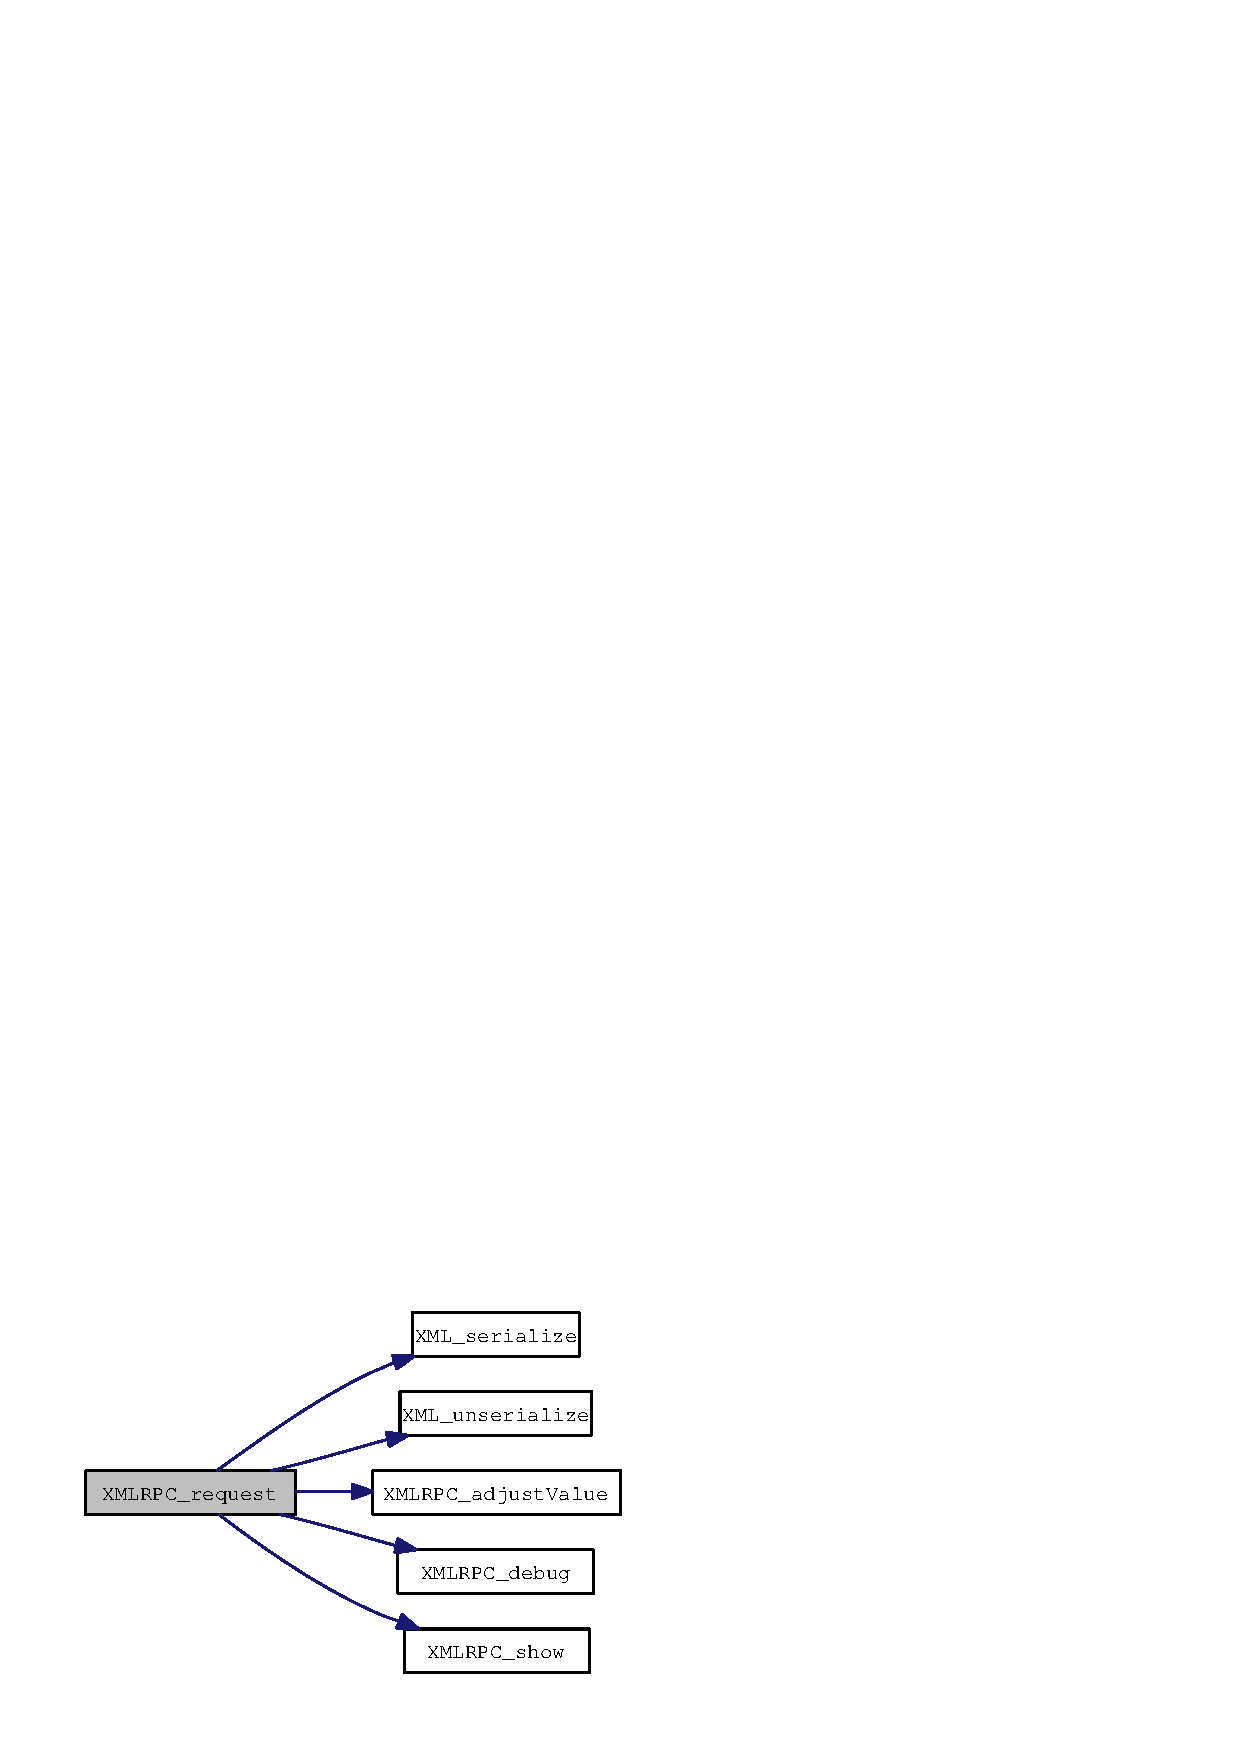
\includegraphics[width=151pt]{xmlrpc_8inc_3a98b6984b8ca01752d1aa9a267526a3_cgraph}
\end{center}
\end{figure}
\hypertarget{xmlrpc_8inc_c736d378caaccdd0726ea1080d1f526f}{
\index{xmlrpc.inc@{xmlrpc.inc}!XMLRPC_response@{XMLRPC\_\-response}}
\index{XMLRPC_response@{XMLRPC\_\-response}!xmlrpc.inc@{xmlrpc.inc}}
\subsubsection{\setlength{\rightskip}{0pt plus 5cm}XMLRPC\_\-response (\$ {\em return\_\-value}, \$ {\em server} = {\tt NULL})}}
\label{xmlrpc_8inc_c736d378caaccdd0726ea1080d1f526f}




Definition at line 418 of file xmlrpc.inc.

References XML\_\-serialize(), XMLRPC\_\-debug(), and XMLRPC\_\-show().

Here is the call graph for this function:\nopagebreak
\begin{figure}[H]
\begin{center}
\leavevmode
\includegraphics[width=141pt]{xmlrpc_8inc_c736d378caaccdd0726ea1080d1f526f_cgraph}
\end{center}
\end{figure}
\hypertarget{xmlrpc_8inc_1f60d2672bcb35f5ff908f64931f8d48}{
\index{xmlrpc.inc@{xmlrpc.inc}!XMLRPC_show@{XMLRPC\_\-show}}
\index{XMLRPC_show@{XMLRPC\_\-show}!xmlrpc.inc@{xmlrpc.inc}}
\subsubsection{\setlength{\rightskip}{0pt plus 5cm}XMLRPC\_\-show (\$ {\em data}, \$ {\em func} = {\tt \char`\"{}print\_\-r\char`\"{}}, \$ {\em return\_\-str} = {\tt false})}}
\label{xmlrpc_8inc_1f60d2672bcb35f5ff908f64931f8d48}




Definition at line 494 of file xmlrpc.inc.

Referenced by XMLRPC\_\-error(), XMLRPC\_\-parse(), XMLRPC\_\-request(), and XMLRPC\_\-response().
\chapter{UPC Lookup Page Documentation}
\input{license}
\hypertarget{todo}{}\section{Todo List}\label{todo}
\label{todo__todo000001}
\hypertarget{todo__todo000001}{}
 \begin{description}
\item[page \hyperlink{index}{Main Page} ]Make this support everyhting Image\_\-Barcode supports:\begin{itemize}
\item Code 39\item Code 128\item EAN 13\begin{itemize}
\item {\bf Done!} \end{itemize}
\item INT 25\item PostNet\begin{itemize}
\item {\bf Will probably not be done, as it can not be read by most barcode scanners and has no practical purpose}\end{itemize}
\item UPCA\begin{itemize}
\item {\bf Done!} \end{itemize}
\end{itemize}


\end{description}

\printindex
\end{document}
